\documentclass[10pt]{beamer}
\usetheme[
%%% options passed to the outer theme
%    hidetitle,           % hide the (short) title in the sidebar
%    hideauthor,          % hide the (short) author in the sidebar
%    hideinstitute,       % hide the (short) institute in the bottom of the sidebar
%    shownavsym,          % show the navigation symbols
%    width=2cm,           % width of the sidebar (default is 2 cm)
%    hideothersubsections,% hide all subsections but the subsections in the current section
%    hideallsubsections,  % hide all subsections
%    right                % right of left position of sidebar (default is right)
  ]{Aalborg}

\definecolor{aaublue}{RGB}{33,26,82}
\definecolor{aaugrey}{RGB}{84,97,110}

% If you want to change the colors of the various elements in the theme, edit and uncomment the following lines
% Change the bar and sidebar colors:
\setbeamercolor{Aalborg}{fg=aaublue!10,bg=aaugrey!60}
%\setbeamercolor{sidebar}{bg=blue!74}
% Change the color of the structural elements:
\setbeamercolor{structure}{fg=aaublue}
 \setbeamercolor{subtitle}{fg=aaugrey}
% Change the frame title text color:
\setbeamercolor{frametitle}{fg=aaublue}
% Change the normal text color background:
%\setbeamercolor{normal text}{bg=aaugrey!10}
% ... and you can of course change a lot more - see the beamer user manual.
\usebackgroundtemplate{
\includegraphics[width=\paperwidth]{img/background}}

\usepackage[utf8]{inputenc}
\usepackage[english]{babel}
\usepackage[T1]{fontenc}
% ... or whatever. Note that the encoding and the font should match. If T1
% does not look nice, try deleting the line with the fontenc.
\usepackage{lmodern} %optional

% colored hyperlinks
\newcommand{\chref}[2]{%
  \href{#1}{{\usebeamercolor[bg]{Aalborg}#2}}
}

\title[Centralized State Estimation\\ of Distributed Maritime Autonomous Surface Oceanographers]% optional, use only with long paper titles
{Centralized State Estimation of Distributed Maritime Autonomous Surface Oceanographers}

%\subtitle[v.\ 0.1.1] %optional
%{v.\ 0.1.1}

\author[Rasmus L. Christensen, Frederik Juul, Nick \O stergaard, Attila Fodor, Tudor Muresan] % optional, use only with lots of authors
{
  Rasmus L. Christensen \and Frederik Juul \and Nick \O stergaard \and Attila Fodor \and Tudor Muresan\\
  {{\tt \{ralch,nickoe,fjuul,afodor12,tmures12\}@es.aau.dk}}
}
% - Give the names in the same order as they appear in the paper.
% - Use the \inst{?} command only if the authors have different
%   affiliation. See the beamer manual for an example

%specify some optional logos
\pgfdeclareimage[height=1.2cm]{mainlogo}{aau_logo.pdf} % placed in the upper left/right corner
\logo{\pgfuseimage{mainlogo}}

\pgfdeclareimage[height=0.75cm]{logo2}{tu-logo} % placed in the lower left/right corner if the \pgfuseimage{logo2} command is uncommented in the \institute command below

\institute[
%  {\pgfuseimage{logo2}}\\ %insert a company or department logo
  Dept.\ of Electronic Systems,\\
  Aalborg University,\\
  Denmark
] % optional - is placed in the bottom of the sidebar on every slide
{%
  Department of Electronic Systems,\\
  Aalborg University,\\
  Denmark
  
  %there must be an empty line above this line - otherwise some unwanted space is added between the university and the country (I do not know why;( )
}
\date{\today}

\begin{document}
% the titlepage
\begin{frame}[plain] % the plain option removes the sidebar and header from the title page
  \titlepage
\end{frame}
%%%%%%%%%%%%%%%%

%###########################

\renewcommand{\vec}[1]{\text{\boldmath$#1$}}

\section{Results}
	\subsection{Kalman filter}
		\begin{frame}{Kalman filter}{Monorate implementation}
			First iteration of the Kalman filter design was a monorate variant. This produced the following results:
			\begin{figure}
				\begin{center}
					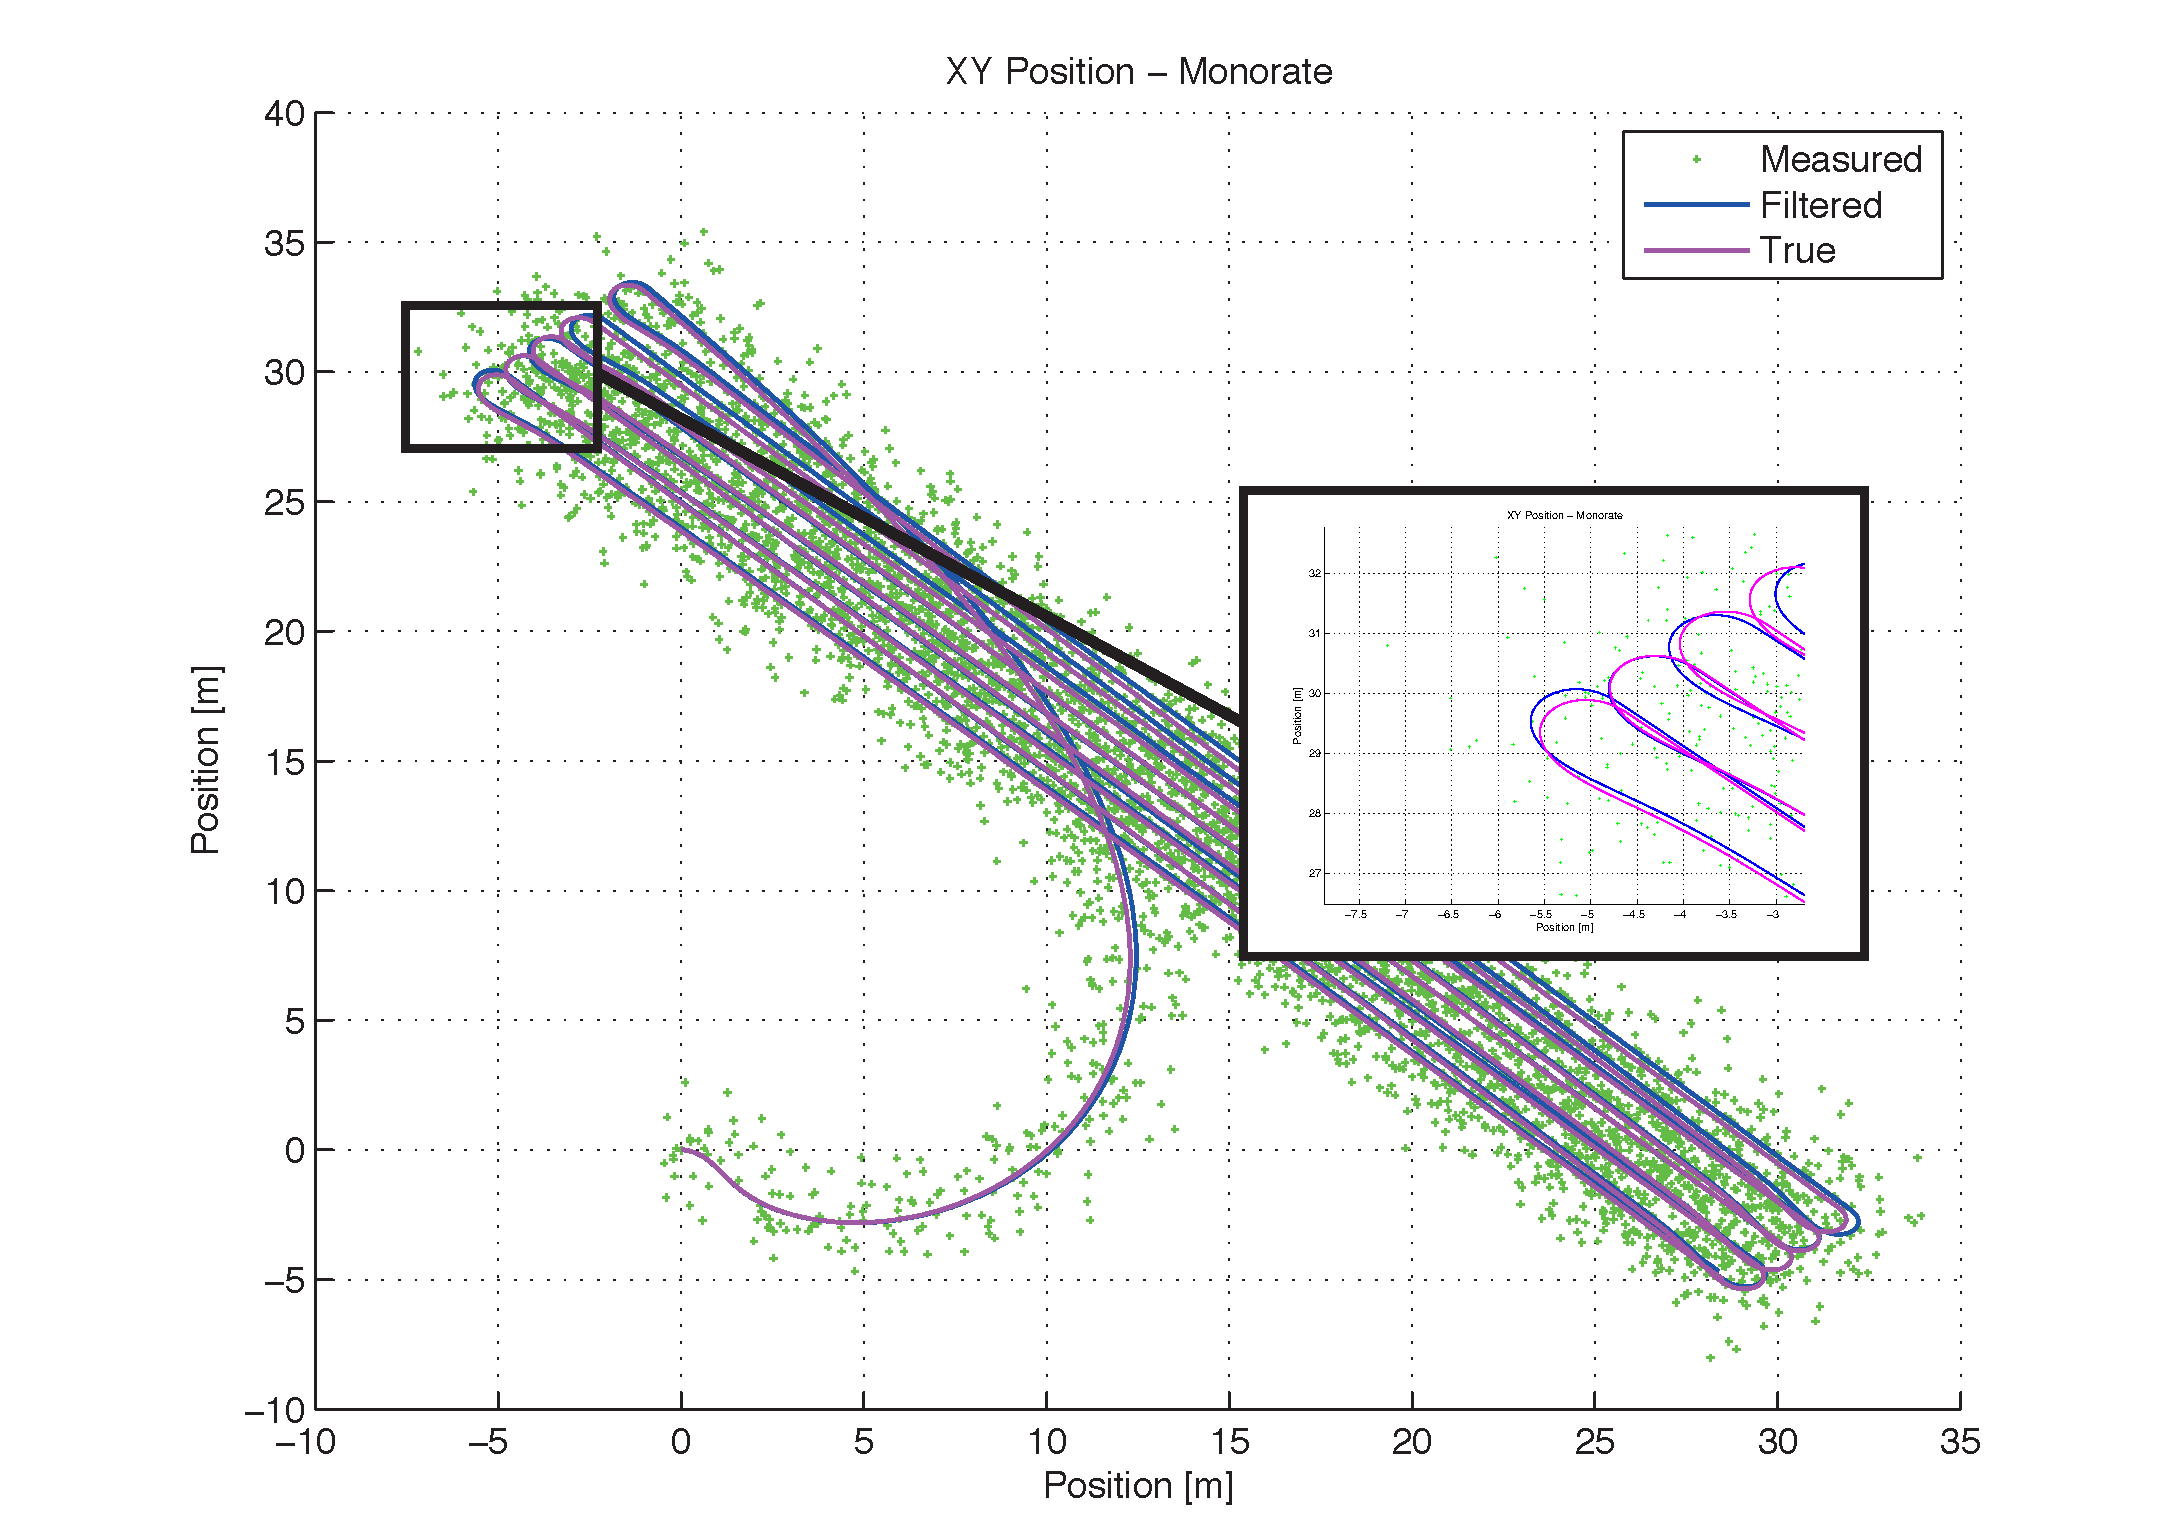
\includegraphics[width=8.2cm]{img/xymono}
					\label{fig:monoratekalman}
				\end{center}
			\end{figure}
		\end{frame}

%###########################

		\begin{frame}{Kalman filter}{Multirate \& input holding}
			\begin{itemize}
				\item The realistic case, using different sampling frequencies
				\item It holds the last GPS position when it does not receive an update
			\end{itemize}
			\begin{figure}
				\begin{center}
					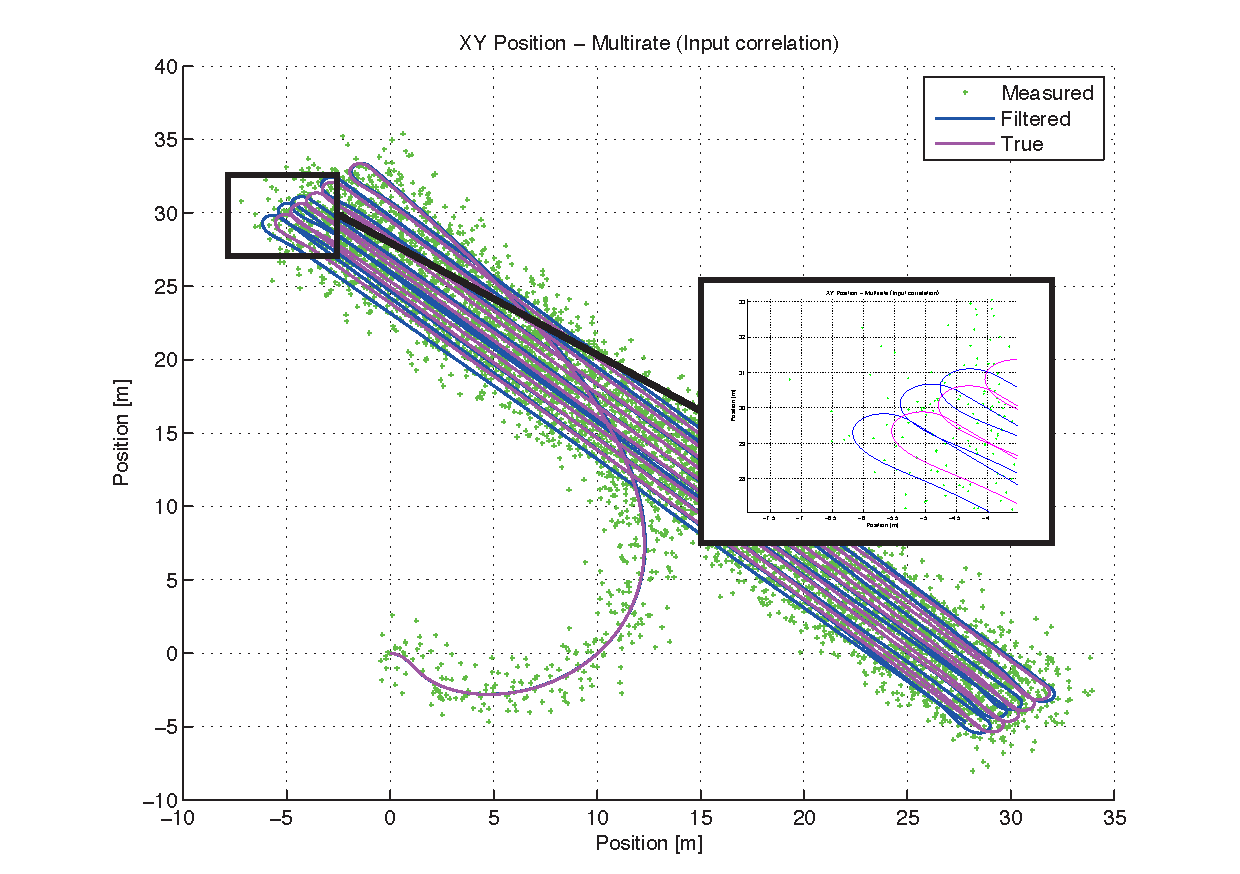
\includegraphics[width=8.2cm]{img/xymnirate}
					\label{fig:multiratekalman1}
				\end{center}
			\end{figure}
		\end{frame}

%###########################

		\begin{frame}{Kalman filter}{Multirate \& input mask}
			The final version: the input mask $ \vec{\Lambda} $ sets the Kalman gain to 0 for invalid inputs.
			\[
		 	\vec{\Lambda} = diag\{\lambda_x,\lambda_{\dot{x}},\lambda_{\ddot{x}},\lambda_{\lambda{y}},\lambda_{\dot{y}},\lambda_{\ddot{y}},\lambda_{\theta},\lambda_{\omega},\lambda_{\alpha} \}
		 	, 
		 	\quad \lambda =  
			 	  \begin{cases}
		 	    1, & \text{valid}\\
		 	    0, & \text{invalid}
			 	  \end{cases}
			\]
			\[
		 	\bar{\vec{K}} = \vec{K} \vec{\Lambda}
		 	\]
			\begin{figure}
				\begin{center}
					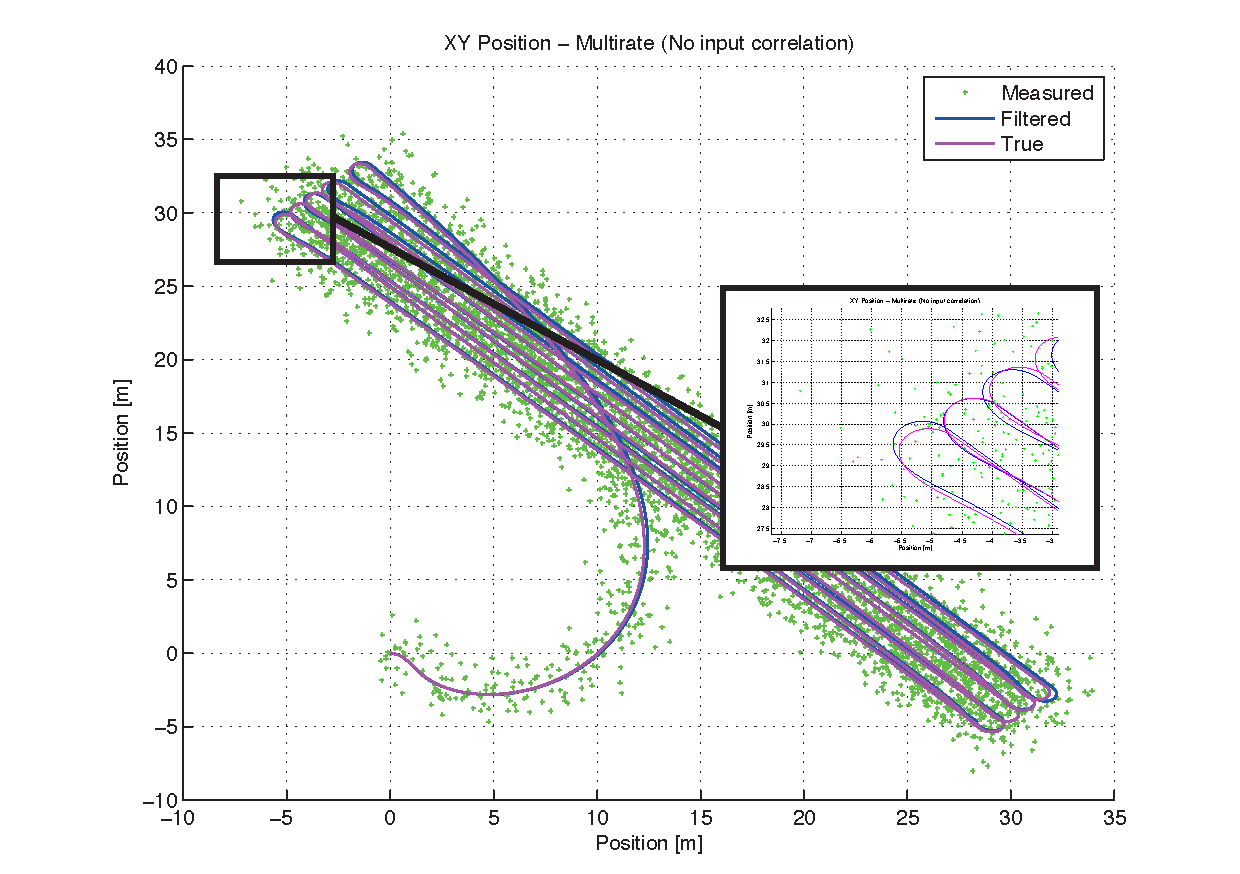
\includegraphics[width=8.2cm]{img/xymultirate}
					\label{fig:multiratekalman2}
				\end{center}
			\end{figure}
		\end{frame}


%###########################

	\subsection{Packet loss}
	% the license
	\begin{frame}{Packet loss}{Considerations}
		\begin{itemize}
			\item<1-> We have a simplex communication link
			\item<2-> It does not guarantee packet arrival or integrity
			\item<3-> It implements a CRC so we can detect errors
			\item<4-> We take advantage of the Kalman filter state estimation
		\end{itemize}
	\end{frame}

%###########################

	\begin{frame}{Packet loss}{Advantages of Kalman filtering}
		\begin{itemize}
			\item Missing GPS samples
			\item Better than simple estimation 
		\end{itemize}
		\begin{figure}
			\begin{center}
				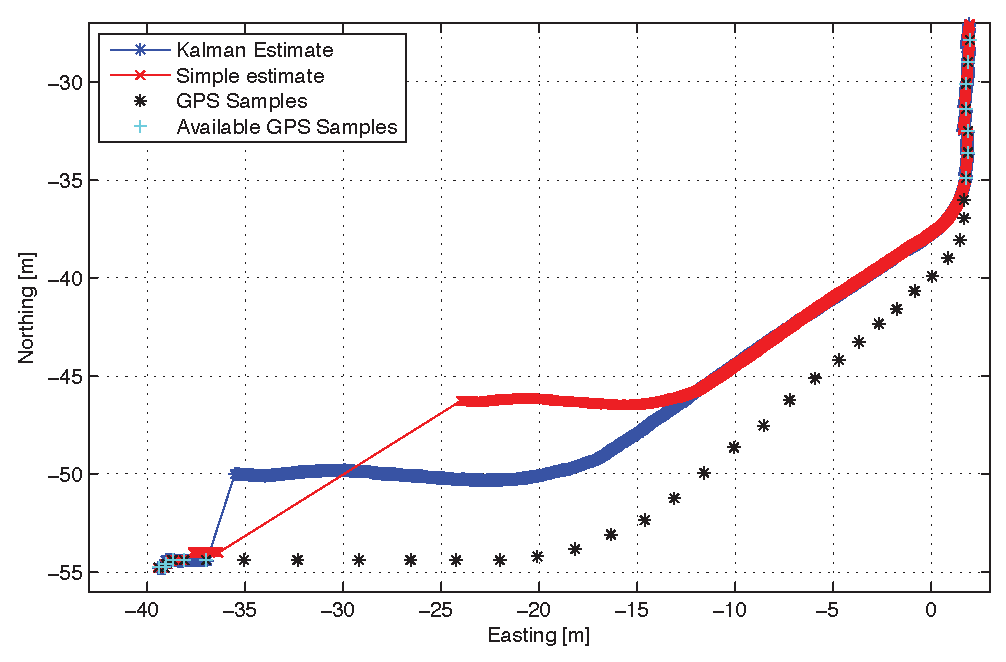
\includegraphics[width=8.2cm]{img/kalmanestimate}
				\label{fig:kalmanestimate}
			\end{center}
		\end{figure}
	\end{frame}
		
%###########################

	\begin{frame}{Packet loss}{Simulation Results}
	  \begin{itemize}
	  	\item Even with and enormously exaggerated packet loss of 100\% for 60 seconds, the Kalman filter still gives a relatively good approximation:
		\begin{figure}
			\begin{center}
				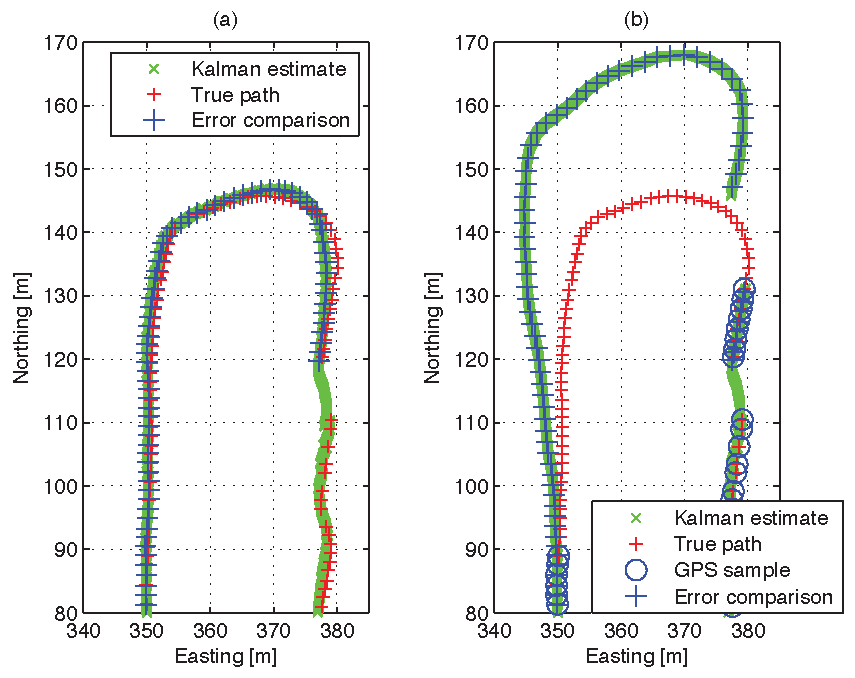
\includegraphics[width=8.2cm]{img/track}
				\label{fig:packetloss}
			\end{center}
		\end{figure}
	  \end{itemize}
	\end{frame}

%###########################

	\begin{frame}{Packet loss}{Simulation Results}
		\begin{itemize}
		  	\item As can be seen, the peak error is around 23 m, which is acceptable
			\begin{figure}
				\begin{center}
					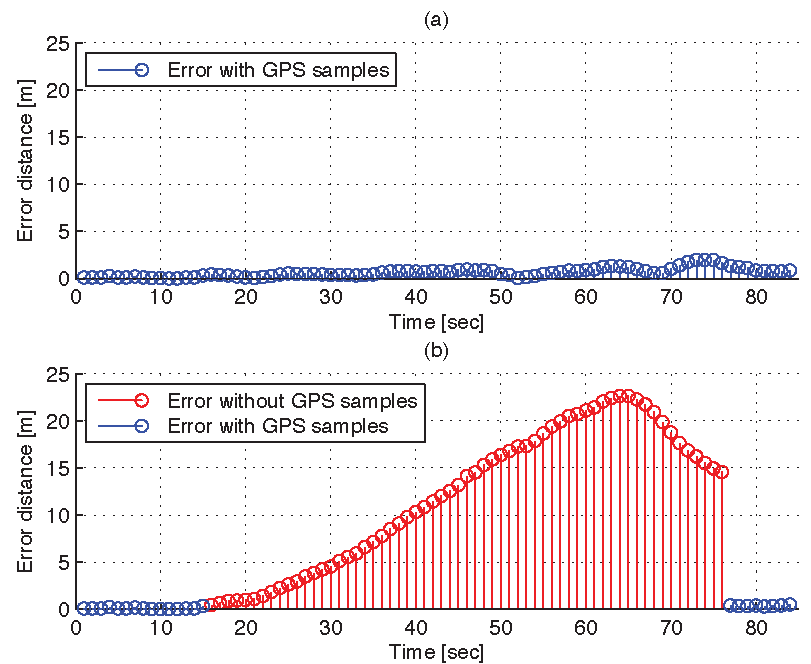
\includegraphics[width=8.2cm]{img/error}
					\label{fig:error}
				\end{center}
			\end{figure}
		\end{itemize}
	\end{frame}

%###########################

	\subsection{Mayden voyage}
	% the license
	\begin{frame}{Mayden voyage}{Purpose and results}
	%  \begin{block}{Ship development}
	  Tested various parts of the ship design and functionality:
	  \begin{itemize}
	  	\item Manual control over wireless link
	  	\item Motor operation and performance
		\item Turning capability and ship stability
		\item Data logging
	  	\end{itemize}
	  	We also added weights to correct its pitch.
	%  \end{block}
		\begin{figure}
			\begin{center}
				\includegraphics[width=9.5cm, trim=0 0 0 50]{img/aauship8}
				\label{fig:aauship}
			\end{center}
		\end{figure}
	\end{frame}

%###########################

	\subsection{Control test}
	\begin{frame}{Testing the control algorithms}{Purpose and results}
		Tested the HLI's waypoint and subwaypoint planning algorithms:
		\begin{itemize}
		\item The ship sailing in Klingenberg lake
		\end{itemize}
		\begin{figure}
			\begin{center}
				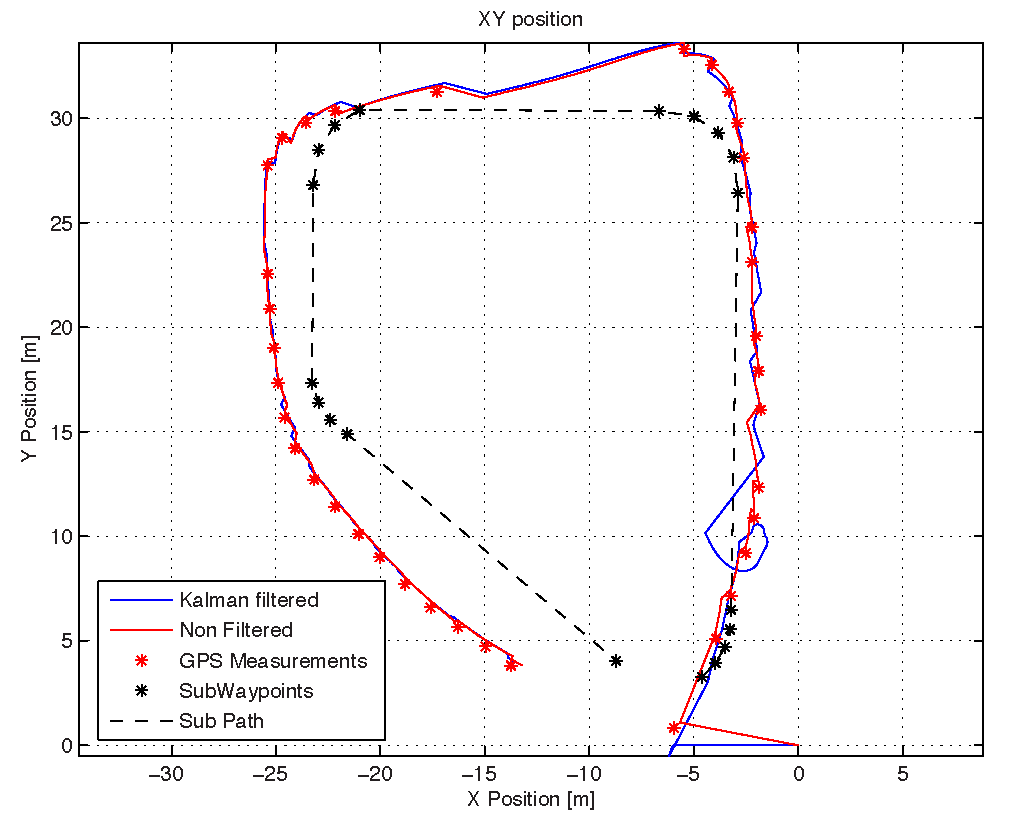
\includegraphics[width=8.2cm]{img/position}
				\label{fig:controltest1}
			\end{center}
		\end{figure}
	\end{frame}

%###########################

	\begin{frame}{Testing the control algorithms}{Results}
		\begin{itemize}
		\item Plot of the ship states during the voyage
		\end{itemize}
		\begin{figure}
			\begin{center}
				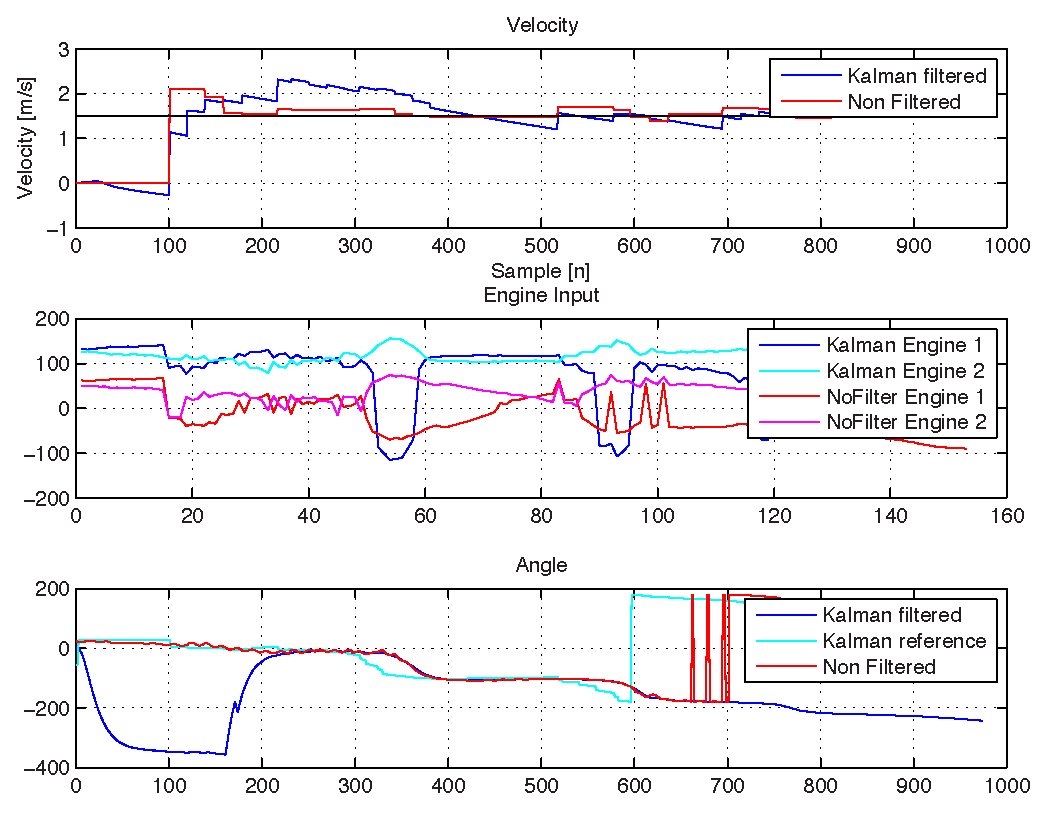
\includegraphics[width=8.2cm]{img/states}
				\label{fig:controltest3}
			\end{center}
		\end{figure}
	\end{frame}

%###########################

	\section{Demonstration}
	\begin{frame}{Demonstration}{}
		Long exposure photo:
		\begin{figure}
			\begin{center}
				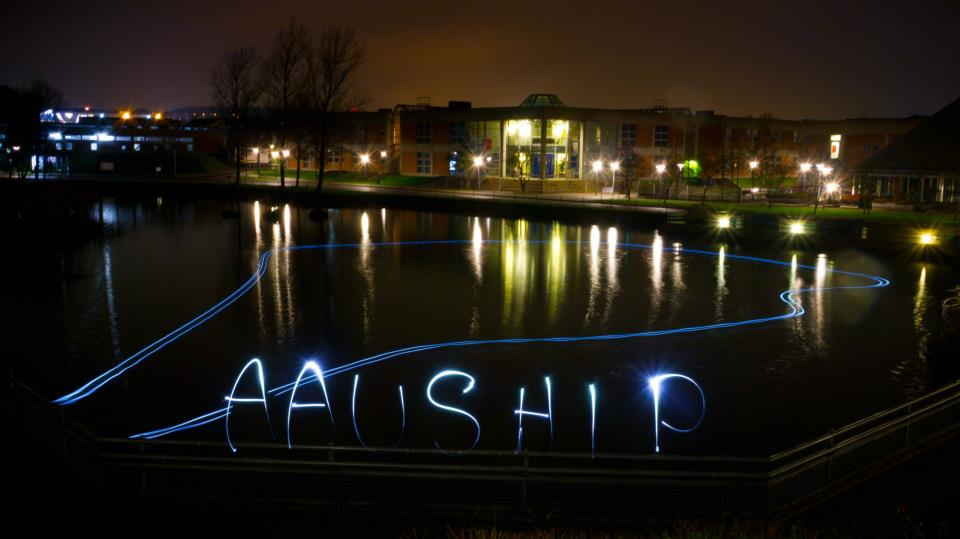
\includegraphics[width=9.6cm]{img/aauship}
				\label{fig:aauship1}
			\end{center}
		\end{figure}
		Next: video of the ship sailing autonomously in lake Klingenberg
	\end{frame}

\end{document}
